\documentclass{article}
\usepackage[utf8]{inputenc}
\usepackage{tikz,graphicx,hyperref,amsmath,amsfonts,amscd,amssymb,bm,cite,epsfig,epsf,url}

\title{MapReduce: Simplified Data Processing
on Large Clusters}
\author{wbg231 }
\date{January 2023}

\begin{document}

\maketitle

\section{Introduction}
\begin{itemize}
    \item a lot of big data applications need to be parallelized, but that used to involve writing a lot of user defined code for tasks that were pretty similar conceptually
    \item map reduce abstracts the parallelization by framing things in terms of a map and reduce structure
    \item apply a map to each record to produce intermediate key value pairs, apply a reduce to all values with a shared key. 
    \item users can define the map and reduce functions 
    \item this model allows for easy parallelization
    \section*{programming model}
    \item map written by user takes an input pair and produces a set of intermediate key/value pairs 
    \item the reduce takes values with the same key and merges these values to form a potentially smaller set of values
    \item consider the task of counting the number of times each word appears in a large document 
    \begin{itemize}
        \item 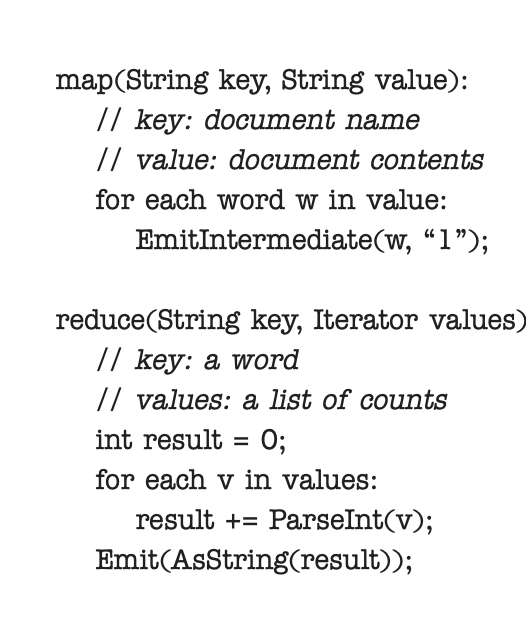
\includegraphics{images/Screenshot 2023-05-08 at 3.10.43 PM.png}
        \item in the above code the map function takes the bag of all words in the document and makes (word,"l") pairs for them 
        \item the reduce function then groups by the key(word) and sums the count 
    \end{itemize}
    \subsection*{implementation}
    \item there are many implementations of map reduce, this is the one originally used at google
    \item the map calls are split across machines by breaking the input data into a set of M splits
    \item the input splits can be worked on in parallel by different machines 
    \item reduce invocations are distributed across many machines by portioning the intermediate key space into R pieces using some partitioning function usually a hash 
    \item the number of partitions (R) is set by the user, so is the partitioning function 
   \item the steps are shown here 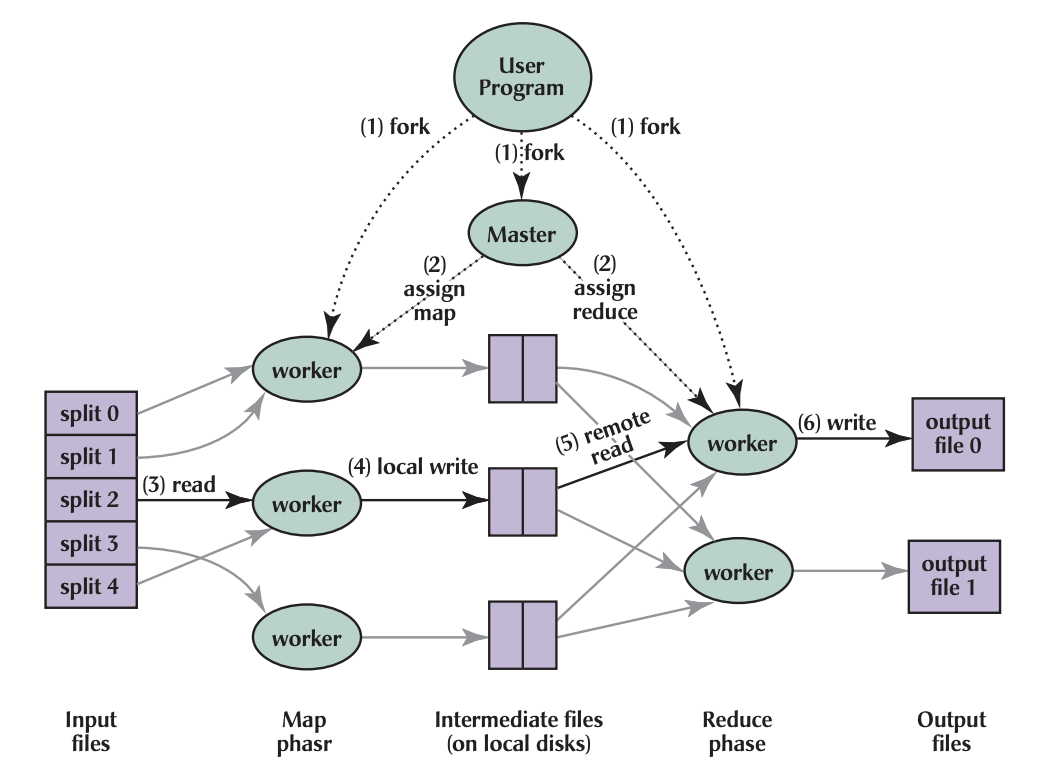
\includegraphics{images/Screenshot 2023-05-08 at 3.18.27 PM.png}
    \begin{enumerate}
        \item map reduce splits the input data into M pieces
        \item one copy of the program is called the master it schedules work the rest are workers that run the map reduce function (the master has to deal with M map tasks and R reduce tasks) the master assigns all idle workers a map or reduce task 
        \item a map worker reads data from the input split, parses key value pairs, passes those key value pairs to the map function to produce intermediate key value pairs that are the buffered into memory
        \item periodically the buffered pairs are written to local disk and partitioned into R regions by the partitioning function 
        \item the reduce worker reads one of the R partitions of the intermediate key value pairs from all the map worker nodes once all data for that partition is read, the reduce worker  sorts by intermediate keys 
        \item the reduce worker than runs the reduce program on each unique intermediate key value, and then appends the output of the reduce function to a final output file. 
        \item when all map tasks and reduce task have been completed the master wakes up teh user program and ends 
    \end{enumerate}
    \item if the program successfully completes the outputs are available in R output files (one for each partition)
    \subsection*{master data structure}
    \item master stores state (idle, in progress , done ) and hte identity of each worker machine 
    \item the master also stores where the values of each partition are for each map worker and then passes it to the reduce worker. 
    \subsection*{fault tolerance}
    \item fault tolerance is a fact of life with this many machines and data 
    \item worker tolerance
     \begin{itemize}
        \item the master node pings workers periodically and if they don't respond for some time there state is set to failed 
        \item after a worker finishes there task there state is set to idle so they can be assigned one of the failed tasks. 
        \item all map tasks ran by a worker that fails must be re-run since workers store intermediate key value pairs locally
        \item when a reducer fails you do not need to re do the reduce calls they have already done since those are written to a file 
        \item when a map tasks fails all reduce tasks that use data from that worker are told and update there data 
        \item this paradigm can handel a lot of worker failure
    \end{itemize}
    \item there are cases where data will be sent to multiple workers, if this is the case the master only pays attention to the first piece of data it gets for this to work the map and reduce functions must be deterministic (this locality is really helpful for speed ups)
    \item map reduce master tries to have map tasks run on distributed machines that have the data they want to work with 
    \subsection*{backup tasks}
    \item the program must wait for all map or reduce functions to finish before moving on so workers that take unusually long hold up the whole Processing
    \item this is basically caused by more keys going to one worker than another called key shift
    \item there are also combine functions that can do partial reduction for keys within the same map task and speed things up in some cases.
    \item the rest of the paper is on performance. 
\end{itemize}
\end{document}
